\documentclass[11pt]{article}
\usepackage[utf8]{inputenc}
\usepackage[french]{babel}
\usepackage[margin=1in]{geometry}
\usepackage{amsfonts, amsmath, amssymb}
\usepackage[none]{hyphenat}
\usepackage{fancyhdr}
\usepackage{graphicx}
\usepackage{float}
\usepackage[nottoc, notlot, notlof]{tocbibind}
\usepackage{array,multirow,makecell}
\setcellgapes{1pt}
\makegapedcells
\usepackage[table]{xcolor}
\usepackage{import}
\usepackage{tikz}
\usepackage{hyperref}
\usepackage{color}
\usepackage{amssymb}

\pagestyle{fancy}
\fancyhead{}
\fancyfoot{}
\fancyhead[L]{\slshape \MakeUppercase{Sur le frottement de la glycérine}}
\fancyhead[R]{\slshape {Julien Bricka, Romain Blondel}}
\fancyfoot[C]{\thepage}
\renewcommand{\footrulewidth}{0pt}

\def \hfillx {\hspace*{ -\textwidth} \hfill}

\setlength\arrayrulewidth{1pt}

\title{\textbf{Sur le frottement de la glycérine}}
\author{Julien Bricka \and Romain Blondel}
\date{1M8, Gymnase Auguste Piccard\\6 Avril 2022}

\begin{document}
    \maketitle

    \section{Introduction}\label{sec:introduction}
Le but de cette expérience est de mesurer le coefficient de viscosité $\eta$ de la glycérine
ainsi que de simuler la vitesse de chute d'une bille en fonction du temps dans cette substance
avec les résultats obtenus. \\
Mais tout d'abord, parlons du coefficient de viscosité dans le modèle des forces de la mécanique
de Newton.
La notion de base, c'est qu'une force est une masse multipliée par son accélération :
$\vec{F} = m \cdot \vec{a}$ en $[N]$ dans les unités du système international.
Les différents facteurs de cette définition sont la masse $m$ en $[Kg]$ et l'accélération $a$ en
$\left[\frac{m}{s^{2}}  \right]$, donc la dérivée de la vitesse en $\left[\frac{m}{s}  \right]$
par rapport au temps, et donc la seconde dérivée de la position en $[m]$
($\vec{a} = \dot{\vec{v}} = \ddot{\vec{x}} $), qui dans un cadre expérimental ou autre
ne nécessitant pas un formalisme mathématiques, peuvent être prise comme une
différence pendant un interval de temps ($ v=\frac{\Delta x}{\Delta t} $
et $a = \frac{\Delta v}{\Delta t} $).
Finalement, il faut noter que la somme des forces d'un système est égal à la masse fois l'accélération
totale du système : $\sum\limits_{i}{\vec{F}_{i}} = m \cdot \vec{a}$. \\
Avec ça, il faut donc lister les forces dans le système expérimental (cf.\ figure~\ref{fig:schemaforce}). \\
\begin{minipage}{0.7\textwidth}
    Les trois forces que l'on va prendre en compte sont : la force pesante
    ($F_{p}=m \cdot g $), la force d'Archimède ($F_{a}=\rho_{liquide}
    \cdot V_{immergé} \cdot g $) et la force de frottement du régime laminaire sur une sphère ($F_{f}=
    K \cdot v $ [cas particulier des équations de Navier-Stokes] où $K = 3 \pi D \eta = 6 \pi R \eta $ avec D et R le diamètre et le rayon de la
    sphère ;
    donc $F_{f} =  6 \pi R \cdot \eta \cdot v $).
    Le coefficient de viscosité $\eta$ n'apparait que dans la force de frottement et est mesurée
    en $\left[N \frac{s}{m^{2}}  \right]  = [Pa \cdot s]$ (décapoise), mais en pratique, on privilégie
    le sous-multiple $1 [mPa \cdot s] = 1 \cdot 10^{-3} [Pa \cdot s]$ (centipoise).
    Sachant que la bille est en acier, son volume vaut $\frac{4}{3}\pi R^{3} $ et donc sa masse
    $\frac{4}{3}\pi R^{3} \cdot \rho_{acier} $.
    On considère la vitesse constante (car la vitesse limite est atteinte, voire section \ref{sec:analyse-des-resultats})
    quand on prend la mesure et donc l'accélération nulle.
    En projetant les forces sur un vecteur unitaire de même sens et direction que $\vec{F}_{p} $,
    la somme vectorielle des forces vaut $F_{p}-F_{a}-F_{f}= m \cdot g - \rho_{glycérine}
    \cdot V_{immergé} \cdot g - 6 \pi R \cdot \eta \cdot v = \frac{4}{3}\pi R^{3} \cdot \rho_{acier}
    \cdot g - \rho_{glycérine} \cdot \frac{4}{3}\pi R^{3} \cdot g - 6 \pi R \cdot \eta \cdot v = 0$.
    De fait,
    \[\eta = \frac{\frac{4}{3}\pi R^{3} \cdot \rho_{acier} \cdot g - \rho_{glycérine} \cdot
    \frac{4}{3}\pi R^{3} \cdot g}{6 \pi R  \cdot v} = \frac{2 R^{2} g (\rho_{acier} - \rho_{glycérine})}
    {v} \]
    Les détails concernant la simulation de la vitesse à travers le temps seront évoqués dans la section
    Résultats (\ref{subsec:simulations}).

\end{minipage}
\begin{minipage}{0.05\textwidth}
\end{minipage}
\begin{minipage}{0.25\textwidth}
    \begin{figure}[H]
        \centering
        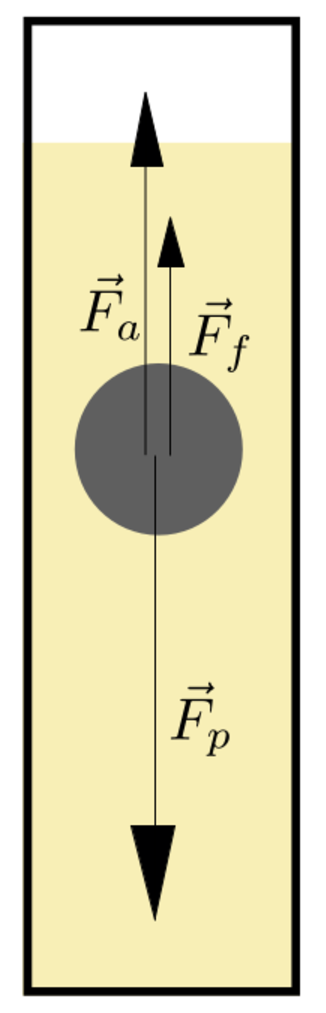
\includegraphics[scale=0.4]{graph/ballinglycsm}
        \caption{Schéma des forces sur une bille dans de la glycérine}
        \label{fig:schemaforce}
    \end{figure}
\end{minipage}
    \section{Démarche}\label{sec:demarche}

\subsection{Matériel}\label{subsec:materiel}
Pour pouvoir réaliser l’expérience nous avons besoin de :
\begin{itemize}
    \item Glycérine
    \item Un cylindre gradué (privilégié une longueur plutôt qu'un gros volume)
    \item De 2 ou 3 billes ayant des rayons différents (en acier dans notre cas)
    \item Un aimant (pour récuperer les billes)
    \item Un entonnoir (pour ne pas verser à côté la glycérine)
    \item Un chronomètre
    \item Un marqueur
\end{itemize}

\subsection{Marche à suivre}\label{subsec:marche-a-suivre}
\begin{enumerate}
    \item Remplir le cylindre gradué de glycérine a l’aide de l’entonnoir et récupérer tous les autres accessoires nécessaires à l’expérience dans le laboratoire (voir matériel).
    \item Tracer deux marques sur le cylindre gradué en utilisant le marqueur.
    Il est conseillé de les tracer à une certaine distance (x = 8.5 [cm] dans notre cas) car le plus écartées sont les marques, le plus les résultats seront fiables.
    Il serait aussi envisageable de ne pas mettre de traces trop hautes non plus, pour ne pas commencer le chronomètre pendant que la bille subit une accélération.
    \item Lâcher la bille au dessus du liquide à l’aide de ses doigts.
    \item Commencer le chronomètre lorsque la bille atteint la première marque puis l’arrêter une fois traversée la deuxième marque.
    \item Prendre note du temps pris pour que la bille fasse x centimètres dans le fluide à vitesse constante.
    \item Récupérer la bille en utilisant l’aimant (le mettre contre le cylindre, et monter jusqu’en haut gentiment lorsque la bille se fait attirer).
    \item Répéter l’expérience plusieurs fois afin d’en faire une moyenne, puis changer le rayon de la bille.
\end{enumerate}

\subsection{Schéma de l'expérience}\label{subsec:schema}
\begin{figure}[H]
    \centering
    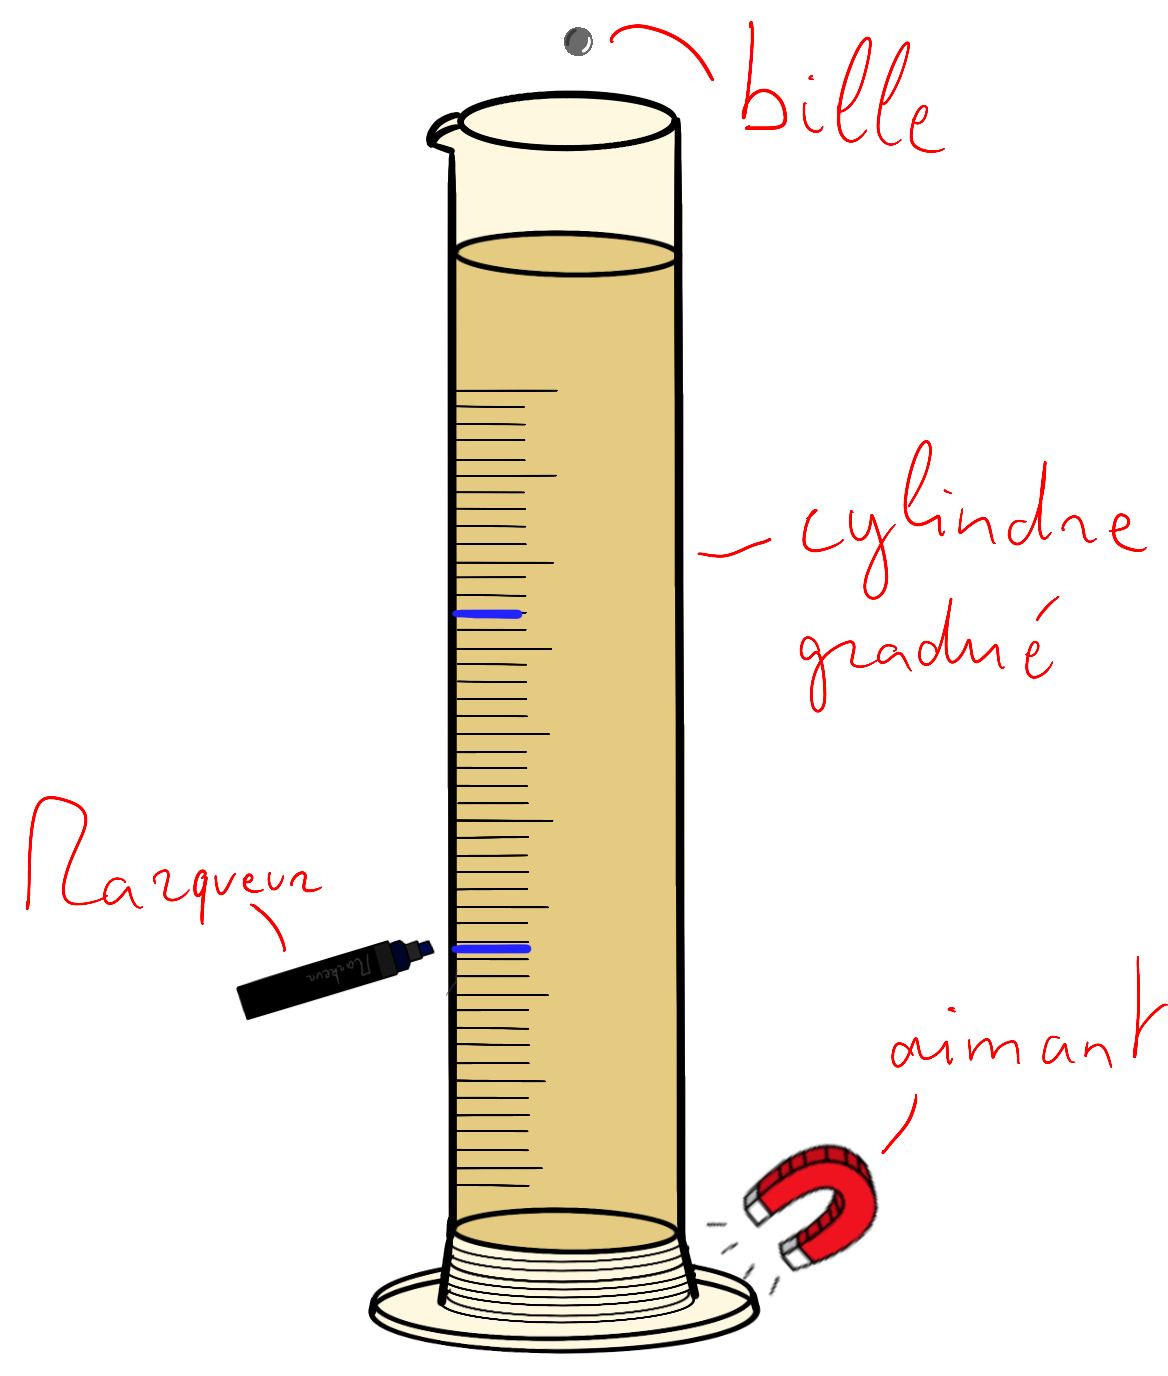
\includegraphics[scale=0.45]{graph/schema-exp}
    \caption{Schéma de l'expérience}
    \label{fig:schema-exp}
\end{figure}
    \section{Résultats}\label{sec:resultats}
Les résultats sont divisés en trois parties : les mesures que l'on a prises ainsi que les constantes
utilisées ;
les calculs effectués afin d'obtenir $\eta $ et finalement les simulations faites de la valeur
de $\eta $.
Toute l'exploitation de ces résultats sera faite dans la section suivante (cf.
section~\ref{sec:analyse-des-resultats}).

\subsection{Mesures}\label{subsec:mesures}
Premièrement, voici les constantes et autres données dont nous avons besoin :
l'accélération terrestre $g= 9.81 \left[ \frac{m}{s^{2}} \right] $, la masse volumique de l'acier
($\rho_{acier} = 7850 \left[ \frac{Kg}{m^{3}} \right] $) et la masse volumique de la glycérine
($\rho_{glycérine} = 1260 \left[ \frac{Kg}{m^{3}} \right] $).
De plus, les trois diamètres différents des billes sont 1, $1.5$ et 2 $[mm]$ soit
$1\cdot 10^{-3}$, $1.5\cdot 10^{-3}$ et $2\cdot 10^{-3}$ $[m]$.
De fait, leurs rayons sont :
\begin{table}[H]
    \centering
    \begin{tabular}{|>{\columncolor{darkgray}} l||l|>{\columncolor{gray}} l|l|}
        \hline
        Diamètre [mm] & 1 & 1.5 & 2 \\
        \hline
        Rayon [m] & $5 \cdot 10^{-4}$ & $7.5\cdot 10^{-4}$ & $1 \cdot 10^{-3}$\\
        \hline
    \end{tabular}
    \caption{Rayon des billes à partir de leur diamètre}
    \label{tab:raybille}
\end{table}
Ensuite, le temps que mets chaque une des billes pour parcourir la distance de $8.5 [cm] = 8.5 \cdot
10^{-2} [m]$ dans la glycérine, mesures réitérées 5 fois par bille :
\begin{table}[H]
    \centering
    \begin{tabular}{|>{\columncolor{darkgray}} l||l|>{\columncolor{gray}} l|l|>{\columncolor{gray}} l|l|}
        \hline
        \rowcolor{darkgray} \cellcolor{black} & $t_{1} [s]$ & $t_{2} [s]$ & $t_{3} [s]$ & $t_{4} [s]$ & $t_{5} [s]$\\
        \hline \hline
        D = 1 [mm] & 4.07 & 4.15 & 4.11 & 4.05 & 4.18\\
        \hline
        D = 1.5 [mm] & 1.63 & 1.83 & 1.74 & 1.88 & 1.77\\
        \hline
        D = 2 [mm] & 1.15 & 1.14 & 1.17 & 1.18 & 1.14\\
        \hline
    \end{tabular}
    \caption{Temps de descente mesuré de chaque bille}
    \label{tab:temps-mesure}
\end{table}

\subsection{Calculs}\label{subsec:calculs}
Pour chaque bille, on a pris la moyenne des temps afin de calculer $\eta$ :
\begin{table}[H]
    \centering
    \begin{tabular}{|>{\columncolor{darkgray}} l||l|>{\columncolor{gray}} l|l|}
        \hline
        Diamètre [mm] & 1 & 1.5 & 2 \\
        \hline
        T [s] & 4.112 & 1.770 & 1.156 \\
        \hline
    \end{tabular}
    \caption{Temps moyens de chute des billes}
    \label{tab:meantime}
\end{table}
Ensuite, on calcule la vitesse de la bille (avec $v= \frac{d}{t} $):
\begin{table}[H]
    \centering
    \begin{tabular}{|>{\columncolor{darkgray}} l||l|>{\columncolor{gray}} l|l|}
        \hline
        Diamètre [mm] & 1 & 1.5 & 2 \\
        \hline
        Vitesse $\left[ \frac{m}{s} \right] $ & $2.067 \cdot 10^{-2}$ & $4.802\cdot 10^{-2}$ & $7.353 \cdot 10^{-2}$\\
        \hline
    \end{tabular}
    \caption{Vitesse des billes selon de leur diamètre}
    \label{tab:vitesse}
\end{table}
Finalement, on calcule $\eta$ avec la formule expliquée dans l'introduction $\eta = \frac{2 R^{2} g (\rho_{acier} - \rho_{glycérine})}
{9 v} $ :
\begin{table}[H]
    \centering
    \begin{tabular}{|>{\columncolor{darkgray}} l||l|>{\columncolor{gray}} l|l|}
        \hline
        Diamètre [mm] & 1 & 1.5 & 2 \\
        \hline
        $\eta$ $[mPs \cdot s ]$ & $173.75$ & $168.27$ & $195.38$\\
        \hline
    \end{tabular}
    \caption{$\eta$ pour chaque bille}
    \label{tab:eta-val}
\end{table}
Donc si l'on prend la moyenne comme valeur pour la suite : $\eta_{moy} \approx 179.13 [mPa \cdot s] $.

\subsection{Simulations}\label{subsec:simulations}
Avec la valeur de $\eta$ obtenue, et en se servant de la somme des forces évoquée en introduction
lorsque la vitesse n'est pas constante $F_{p}-F_{a}-F_{f}=m \cdot a$, on va faire des simulations
de l'évolution de la vitesse en fonction du temps selon le rayon de la bille et de la vitesse
initiale ($v_{0}$).
\subsubsection{Itératives}
Première méthode pour faire ces simulations : prendre un interval de temps, calculer la vitesse en
$t_{i+1}$ avec l'accélération en $t$ via un MRUA ($v(t) = v_{0} + a \cdot t $) et l'accélération
en $t_{i+1}$ via la vitesse précédement calculée par la somme des forces
$\frac{4}{3}\pi R^{3} \cdot \rho_{acier} \cdot g - \rho_{glycérine} \cdot \frac{4}{3}\pi R^{3}
\cdot g - 6 \pi R \cdot \eta \cdot v =  \frac{4}{3}\pi R^{3} \cdot \rho_{acier} \cdot a \Longleftrightarrow a =
\frac{g (\rho_{acier}-\rho_{glycérine})}{\rho_{acier}} - \frac{9 \eta }{2 R_{2} \rho_{acier}}\cdot v
= A - B \cdot v $ (les grosses valeurs constantes ont été substituées par A et B ; sur les graphes,
on nomme les courbes selon leur $v_{0}$).
\begin{minipage}{0.475\textwidth}
    \begin{figure}[H]
        \centering
        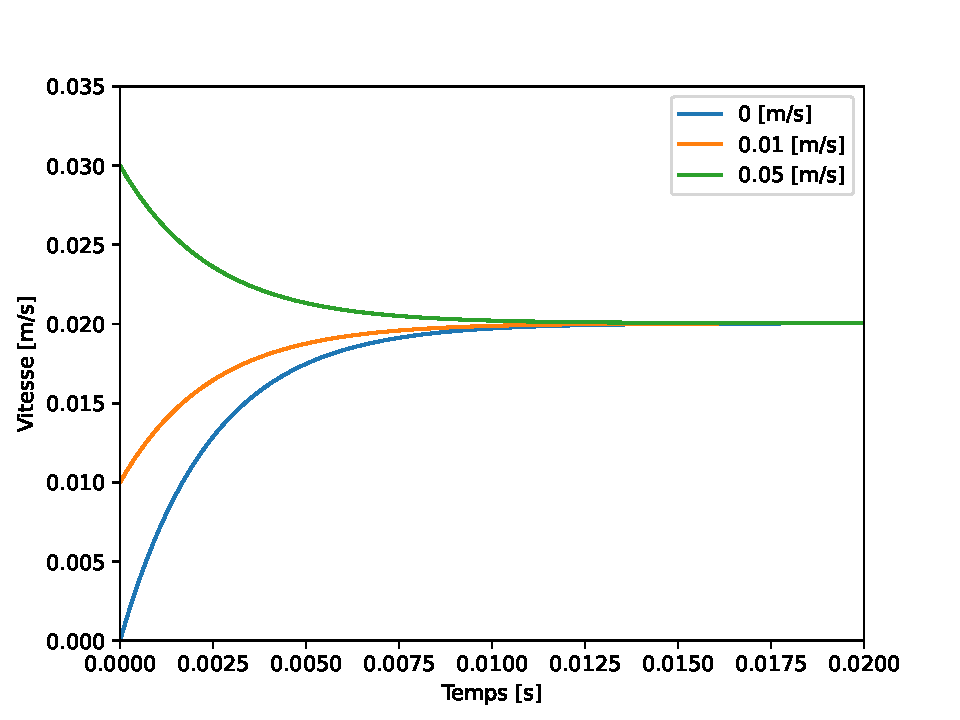
\includegraphics[scale=0.55]{graph/ray1_it}
        \caption{Vitesse pour une bille de 1 [mm] de diamètre}
        \label{fig:ray1_it}
    \end{figure}
\end{minipage}
\begin{minipage}{0.05\textwidth}
\end{minipage}
\begin{minipage}{0.475\textwidth}
    \begin{figure}[H]
        \centering
        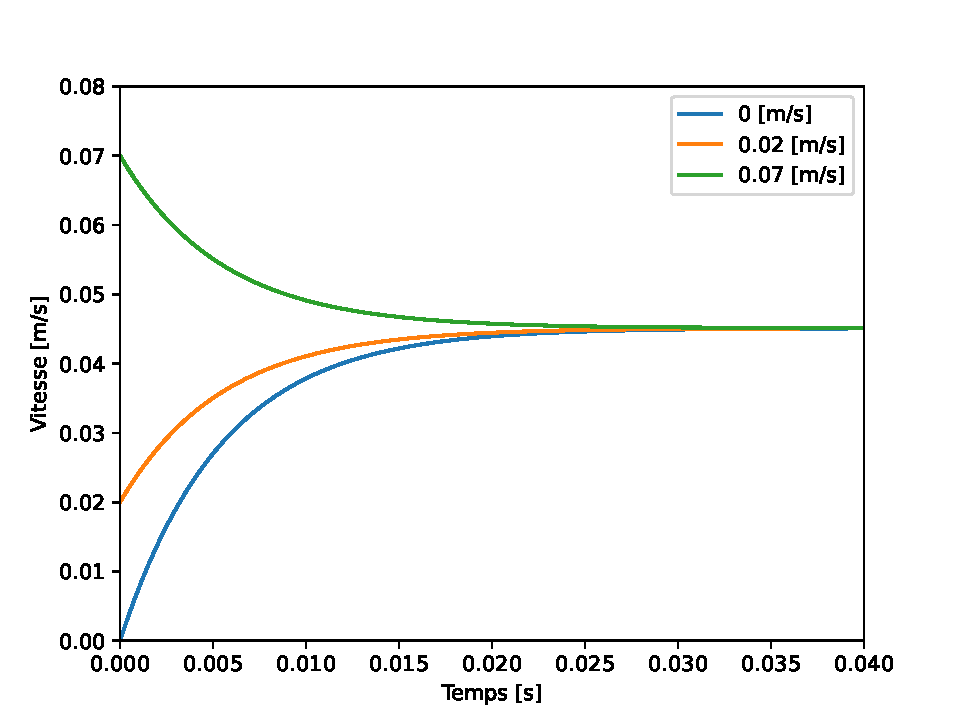
\includegraphics[scale=0.55]{graph/ray2_it}
        \caption{Vitesse pour une bille de 1.5 [mm] de diamètre}
        \label{fig:ray2_it}
    \end{figure}
\end{minipage}
\begin{figure}[H]
    \centering
    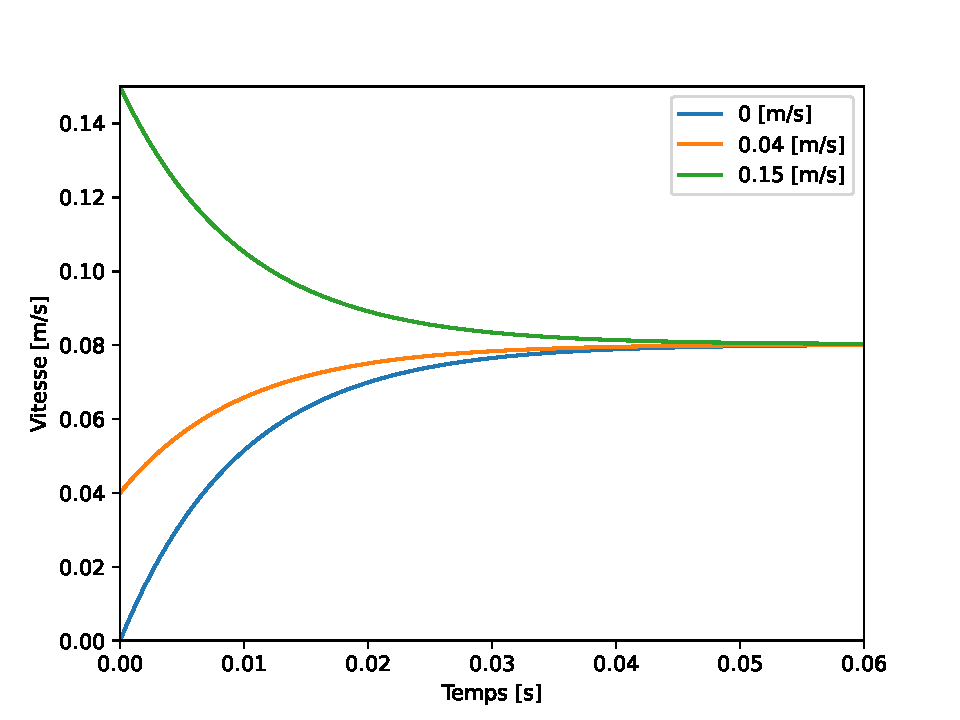
\includegraphics[scale=0.55]{graph/ray3_it}
    \caption{Vitesse pour une bille de 2 [mm] de diamètre}
    \label{fig:ray3_it}
\end{figure}

\subsubsection{Autres}
Comme autre méthode, on peut résoudre mathématiquement l'équation différentielle \footnote{Note :
la résolution d'équation différentielle est faite via "Wolfram Alpha" car on ne maitrise pas très
bien ces outils. Néanmoins, les dérivées et intégrales en section~\ref{sec:analyse-des-resultats} sont juste
verifiée avec ce logiciel.} $a(t)= v'(t) = A - B \cdot v(t) \Longleftrightarrow v(t) = \frac{A}{B}+c \cdot
e^{-B\cdot t} $ où $c$ est une constante que l'on peut calculer vu que l'on connait $v_{0}$
($t=0$, donc $v_{0} = \frac{A}{B}+c \Longleftrightarrow c = v_{0}- \frac{A}{B}$)[cf.\ figure~\ref{fig:ray3_th}].\\
En prenant beaucoup de valeurs $v_{0}$ de départ, on peut également faire une image de la densité de
points qui illustre bien la convergence de la vitesse en une limite [cf.\ figure~\ref{fig:densplot}].\\
\begin{minipage}{0.475\textwidth}
    \begin{figure}[H]
        \centering
        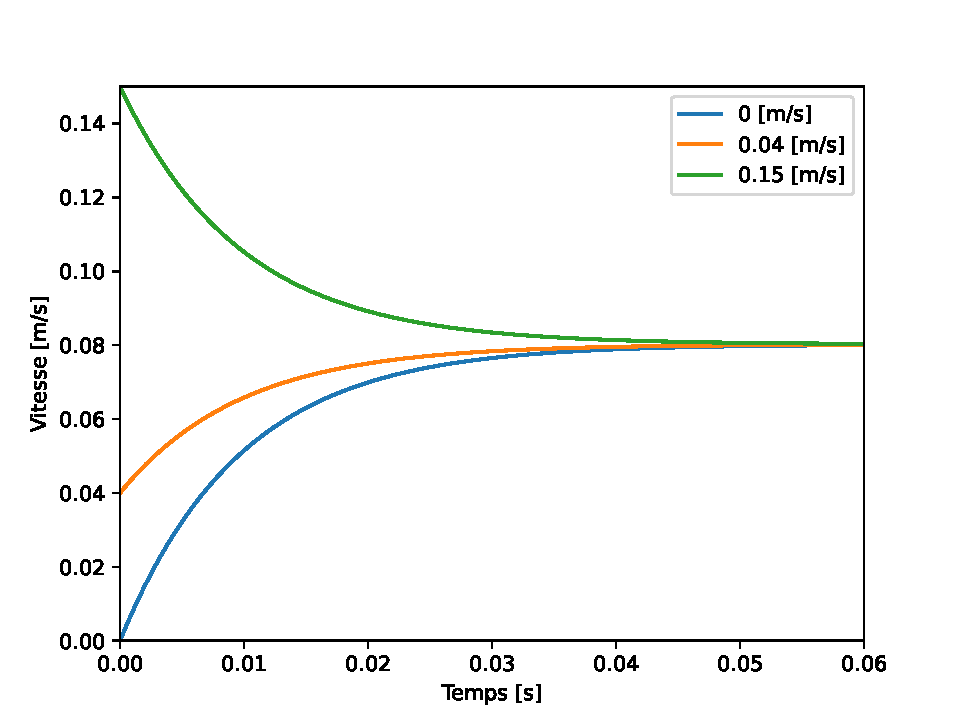
\includegraphics[scale=0.54]{graph/ray3_th}
        \caption{Vitesse pour une bille de 2 [mm] de diamètre avec la fonction théorique}
        \label{fig:ray3_th}
    \end{figure}
\end{minipage}
\begin{minipage}{0.05\textwidth}
\end{minipage}
\begin{minipage}{0.475\textwidth}
    \begin{figure}[H]
        \centering
        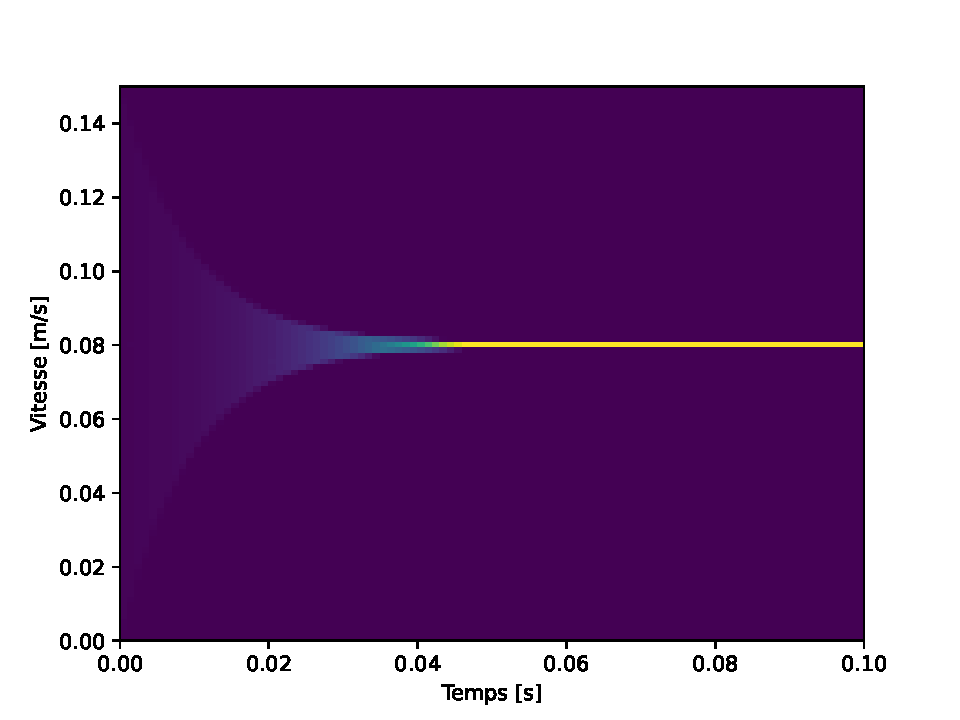
\includegraphics[scale=0.54]{graph/densplot}
        \caption{"Densité" de la vitesse en fonction du temps pour une bille de 2 [mm] de diamètre}
        \label{fig:densplot}
    \end{figure}
\end{minipage}

    \section{Analyse des résultats}\label{sec:analyse-des-resultats}
Premièrement, on constate dans la table~\ref{tab:eta-val} que plus la bille est petite, plus son
temps de chute est lent (la valeur de $\eta$ obtenue pour la bille 1 [mm] est entre les deux autres),
et donc plus la mesure est précise ;
néanmoins, cette précision peut en partie être contrebalancée par celle dans la mesure de la bille qui
sera moindre.
On constate ça également avec les graphes et tables de vitesses qui montrent que plus la bille est petite,
plus elle va lentement. \\
Ensuite, on constate que les simulations correspondent bien aux mesures, en comparant
les vitesses dans la table~\ref{tab:vitesse} avec les graphes des figures~\ref{fig:ray1_it}, ~\ref{fig:ray2_it} et~\ref{fig:ray3_th} : les valeurs de la table correspondent à peu près (à cause
des arrondis sur $\eta$) à l'endroit où convergent/tendent les graphes de vitesse.
De plus, cela confirme le concept de vitesse limite que nous laissait percevoir le modèle des forces :
la force pesante étant plus grande que la force d'Archimède et les deux étant constante ;
de fait, seul la force de frottement va varier en s'opposant au mouvement de la bille qui coule.
Pour conclure, lorsque la somme des forces est nul, la vitesse limite est atteinte.
Comme on le voit sur les graphes, il ne faut pas longtemps à la bille pour y arriver.
\\
Toujours en parlant de fonction, on voit que la résolution "litérale" correspond à la méthode
itérative.
En effet, la figure~\ref{fig:ray3_th} est la même que celle~\ref{fig:ray3_it}. \\
De plus, cette fonction théorique nous indique que la vitesse est une fonction exponentielle du
temps, et de fait on peut connaitre la fonction de l'accélération $a(t)= \frac{d}{dt} \left( \frac{A}{B}+c \cdot
e^{-B\cdot t} \right)= -B\cdot c\cdot e^{-B \cdot t} $ et la fonction de la position
$ x(t) = \int \frac{A}{B}+c \cdot e^{-B\cdot t} dt = \frac{A \cdot t - c \cdot e^{-B\cdot t}}{B} + c_{1} $
où $c$ est la constante définie dans la section~\ref{subsec:simulations} et $c_{1}$ une autre constante
liée à l'intégrale, que l'on peut calculer de la même manière que $c$ en connaissant $x_{0}$ dans ce cas.\\
Le diagramme en figure~\ref{fig:densplot} illustre aussi la convergence quelle que soit la vitesse
initiale (les zones violettes sont celles avec le moins de points et plus il y en a, plus ça tend vers
le jaune). \\
Finalement, on peut grâce à la valeur d'$\eta$ trouvée estimer la concentration en glycérine de la
solution utilisée via la table~\ref{tab:table-viscu} : $\sim 85-90 \%$.

\begin{table}[H]
    \centering
    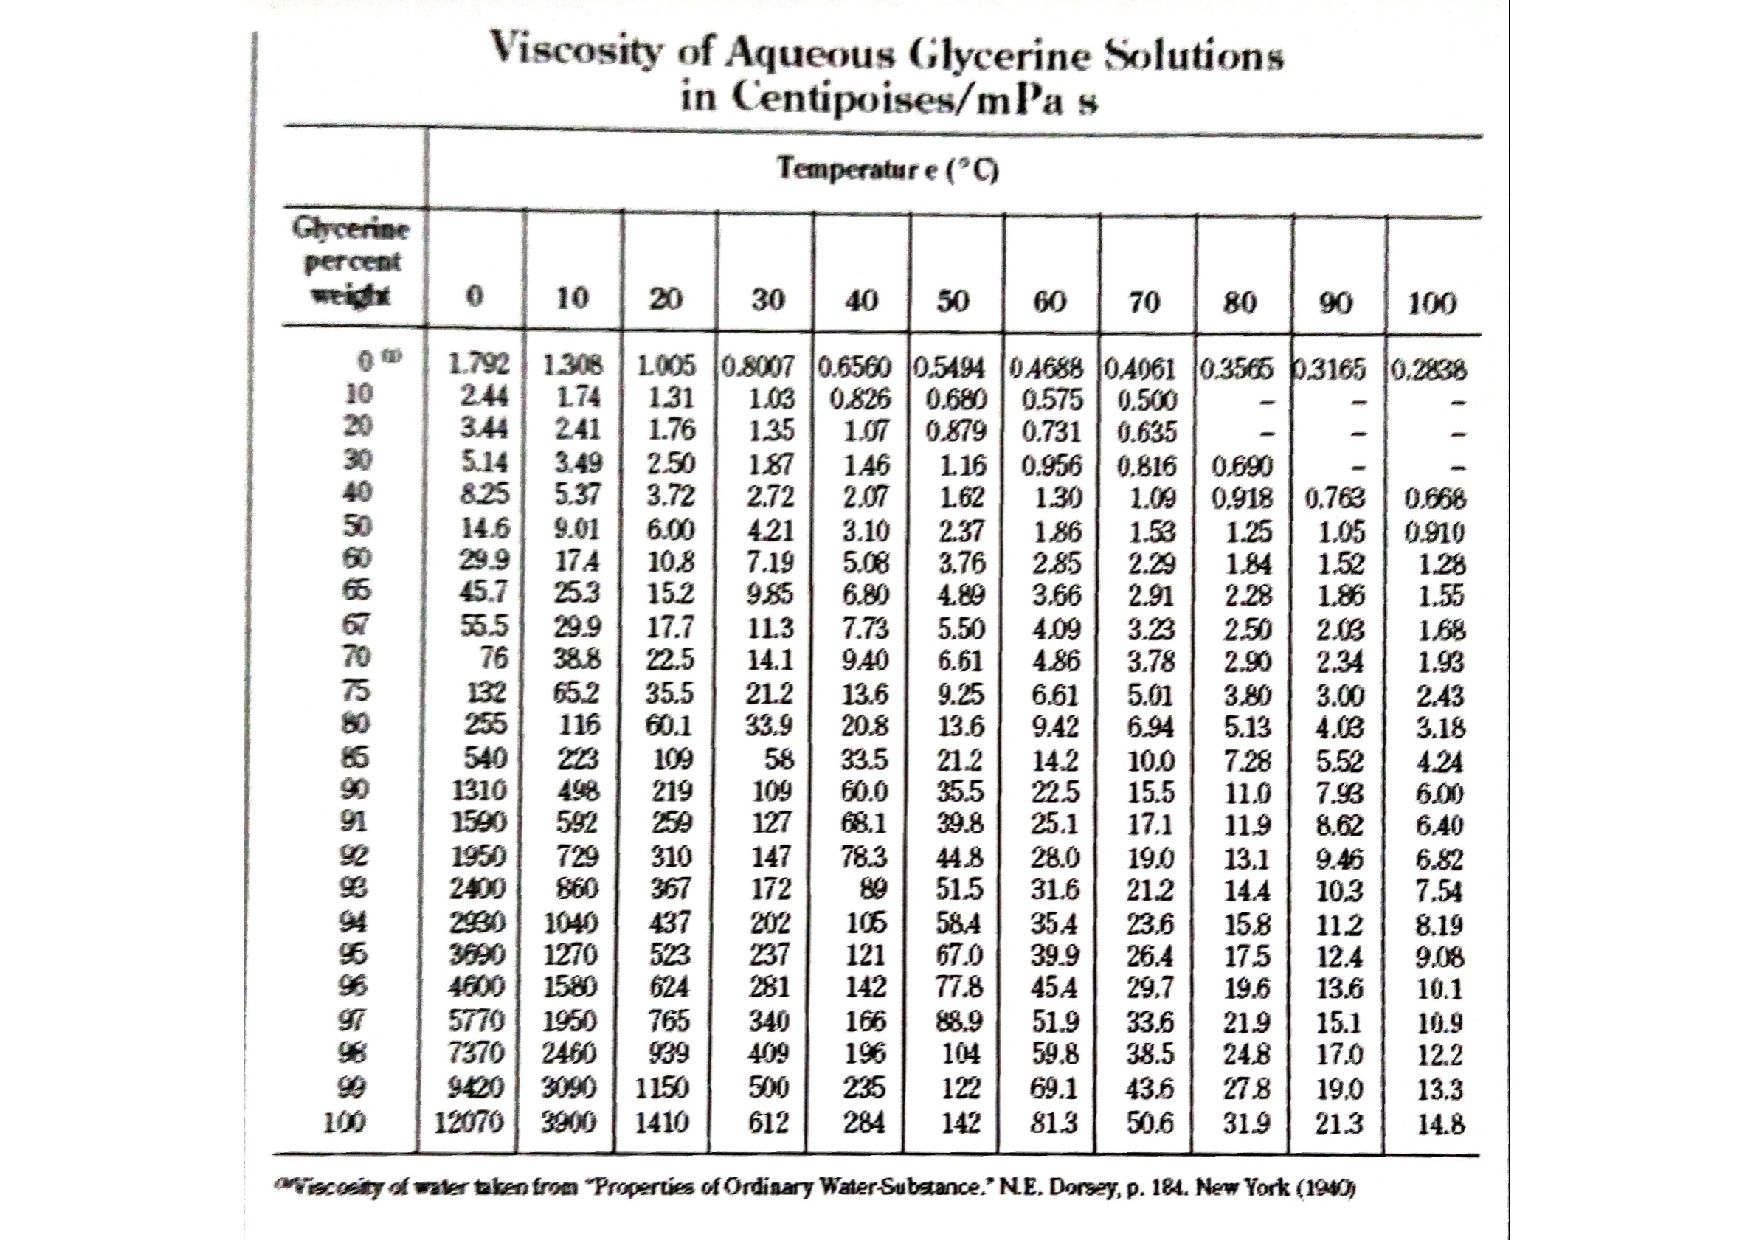
\includegraphics[scale=0.5]{graph/table-viscu}
    \caption{Viscosité d'un mélange eau-glycérine en fonction de sa concentration}
    \label{tab:table-viscu}
\end{table}
    \section{Conclusion}\label{sec:conclusion}
L'expérience s'avère concluante : une valeur plausible comme coefficient de viscosité à été trouvée,
puis les simulations sont cohérentes quelles que soient les méthodes.
Néanmoins, il faut noter une incertitude non négligeable sur les mesures : les marques sur le tube,
ainsi que la mesure de leur distance n'est pas très précise ;
l'observateur peut être perturbé par l'image de la bille dans la glycérine qui se voit
via les effets optiques de diffraction par exemple (et autres effets de perspectives) ;
ainsi que les incertitudes négligeables tels que ceux lié au modèle utilisé.
L'expérience peut être exploitée différement et de manière peut-être plus précise via une vidéo de
la chute de la bille puis une analyse sur un logiciel adapté.
Pour conclure, nous sommes satisfaits des résultats obtenus et des exploitations possibles de
l'expérience via par exemple les simulations de vitesse effectuées.

\end{document}
